\section{Übersicht der Pipeline}\label{sec:ml_pipeline}


Abbildung \ref{fig:ml_pipeline} zeigt den Aufbau der typischen Pipeline, um ein neuronales Netz zu trainieren. 
Diese wird im Folgenden genauer beschrieben.
Schritt 1 umfasst die Vorverarbeitung der Daten.
Es wird angenommen, dass die Daten bereits gesammelt sind und in einer Datenbank abgelegt sind.
Die Vorverarbeitung der Daten ist recht individuell und kann je nach Anwendungsfall variieren. 
Typische Handlungen sind:
\begin{compactitem}
\item Vereinheitlichung des Datenformats
\item Entfernen von starken Ausreißer und Fehlern
\item Normalisierung der Daten
\item Erstellung neuer Daten durch Transformationen
\item Kodierung von kategorialen Variablen und Labels
\item Aufteilung in Trainings-, Validierungs- und Testdatenmengen
\end{compactitem}
\begin{figure}[!htb]
    \centering
    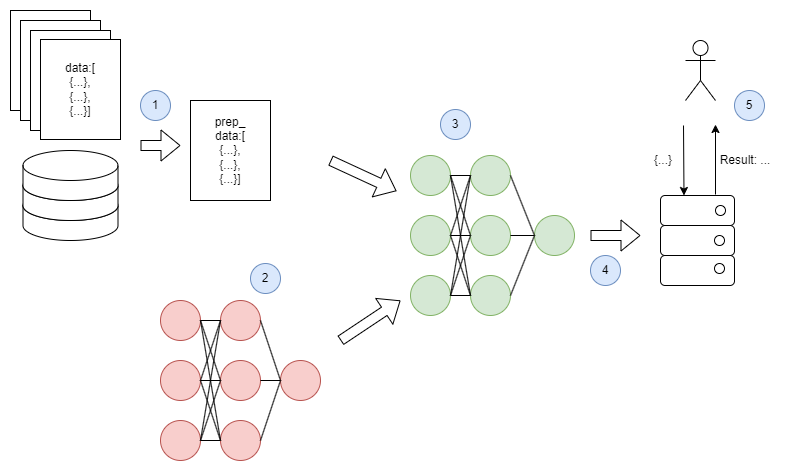
\includegraphics[width=14cm]{figures/ml_pipeline.png}
    \caption{Training eines neuronalen Netzes}
    \label{fig:ml_pipeline}
\end{figure} 

Abbildung \ref{fig:ml_pipeline} stellt die Vorverarbeitung in einem Schritt dar, bei welchem mehrere Datenquellen verbunden werden und nur ein Dokument übrig bleibt. 
Dieses eine Dokument soll zeigen, dass nur die wichtigen Informationen der Daten erhalten bleiben, jedoch kann es in der Praxis sein, dass die Datenmenge beim Aufbereiten der Daten größer wird. 
Kapitel \ref{sec:training_modells} stellt verschiedene Methoden vor, die bei der Vorverarbeitung der Daten angewendet werden können, um die Vertraulichkeit zu sichern.

Schritt 2 umfasst die Architektur eines Modells.
Je nach Anwendungsfall und Komplexität der Aufgabe werden unterschiedliche Konfigurationen der einzelnen Schichten eines neuronalen Netzes vorgenommen.
Dabei werden die Gewichte zufällig oder anhand einer definierten Verteilung initialisiert.
In der Abbildung wird dies durch ein rotes Modell angezeigt, da die Gewichte des Modells noch nicht trainiert sind und demnach keine sinnvollen Vorhersagen getroffen werden können.
Schritt 3 ist der tatsächliche Trainingsvorgang, bei dem das untrainierte Modell lernt.
Grob lässt sich das Training in folgende Schritte einteilen, die mehrfach mit jedem Datenpunkt durchgeführt werden können:
\begin{compactenum}
\item \textbf{Forward-Pass: }Ein Datensatz oder mehrere gebündelte Datensätze, auch Batch genannt, werden durch das Modell gegeben, wodurch eine Vorhersage berechnet wird. 
Dies wird auch Inferenz genannt.
\item \textbf{Backpropagation: }Die Abweichung von der tatsächlichen Vorhersage zu dem Label des Datensatzes wird mittels einer Verlustfunktion quantifiziert. Mittels dieses Wertes der Verlustfunktion lassen sich Gradienten für die Gewichte des neuronalen Netzes berechnen. Diese bestimmen die Richtung der Anpassung der aktuellen Gewichte, wohingegen die Lernrate die Intensität der Anpassung bestimmt.
\end{compactenum}
Ein Durchgang der obigen Schritte mit jedem Datensatz der Trainingsdatenmenge wird dabei Epoche genannt. 
Um den Trainingsfortschritt zu beobachten, kann eine Epoche zusätzlich auch eine Evaluierung mittels einer Validierungsdatenmenge enthalten.
In der Praxis können zusätzliche Schritte in das Training einer Epoche integriert werden, wie ein erweitertes Logging oder eine zusätzliche Überwachung.
Die optimale Anzahl an Epochen ist dabei für jedes Modell unterschiedlich.
Grafisch wird das Training in Abbildung \ref{fig:ml_pipeline} durch den Verbund der Datenmenge und des untrainierten, roten Modells dargestellt. 
Es entsteht ein grünes Modell, welches in der Lage ist, sinnvolle Vorhersagen zu erzeugen.
Kapitel \ref{sec:training_modells} widmet sich Methoden, die während des Trainings, welche aus Schritt 2 und 3 besteht, angewendet werden.

Schritt 4 und 5 beschreiben das Deployment und den Betrieb des Modells. 
Das Ziel dieser Schritte ist es, ein trainiertes neuronales Netz für die vorgesehenen Anwender zur Verfügung zu stellen.
Je nach Anwendungsfall kann die Systemarchitektur unterschiedlich aussehen. 
Einige Modelle werden mit Trainingscode auf öffentlichen Plattformen, wie HuggingFace\footnote{https://huggingface.co/models}, geteilt, wohingegen andere Modelle, wie ChatGPT\footnote{https://chat.openai.com/}, nur über eine spezielle Oberfläche erreichbar sind.
Abbildung \ref{fig:ml_pipeline} zeigt deshalb lediglich einen Anwender, der direkt einen Request an das Modell schickt.
In Kapitel \ref{sec:betrieb} werden Maßnahmen besprochen, die in dieser Phase die Vertraulichkeit sichern. 
Dabei kann es sich um Transformationen des Modells vor dem Deployment handeln, oder um Mechanismen, die Anfragen und Antworten des Modells abwandeln.